\documentclass[10pt,a4paper]{article}
\usepackage[T1]{fontenc}
\usepackage[utf8]{inputenc}
\usepackage{lmodern}
\usepackage[margin=1.9cm]{geometry}
\usepackage{amsmath}
\usepackage{booktabs}
\usepackage{graphicx}
\usepackage{float}
\usepackage{tikz}
\usetikzlibrary{positioning}
\usepackage{caption}
\usepackage{enumitem}
\usepackage{titlesec}
\usepackage[hidelinks]{hyperref}

\captionsetup{font=small,labelfont=bf,skip=3pt}
\titlespacing*{\section}{0pt}{1.4ex plus .3ex}{0.6ex}
\titlespacing*{\subsection}{0pt}{1.0ex plus .2ex}{0.4ex}
\setlength{\parskip}{0.35ex}
\setlength{\parindent}{0pt}
\setlength{\emergencystretch}{2em}
\setlist[itemize]{leftmargin=1.2em,itemsep=0.2ex,topsep=0.3ex}

\newcommand{\feat}[1]{\texttt{\detokenize{#1}}}

\title{\vspace{-1.2cm}\large Tugas 3: Penyempurnaan Model dan Integrasi Multimodal\\[2pt]
\large Prediksi Log Return USD/IDR dengan Fusion Kurs dan Embedding Berita}
\author{}
\date{}

\begin{document}
\maketitle
\vspace{-1.4cm}

\section{Ringkasan}
Laporan ini membandingkan tiga tingkat representasi teks pada target yang sama, yaitu log return kurs tengah USD/IDR hari berikutnya. Model A hanya memakai tujuh fitur kurs. Model B menambahkan sentimen lexicon Tugas 2 (VADER dan Loughran-McDonald). Model C menambahkan embedding transformer dari judul berita, dengan dua skema fusion: early fusion (gabung fitur sebelum regresi) dan late fusion (gabung prediksi dua model unimodal). Semua varian memakai 836 hari latih, 178 hari validasi, dan 180 hari uji, dengan scaler dan PCA hanya di-fit pada data latih. Hasil terbaik adalah \textbf{C\_combined} (Random Forest, 135 fitur) dengan RMSE uji 0,002835 dan Direction Accuracy 0,591, sekitar 4,9\% lebih rendah daripada Model A. Namun baseline naif ``prediksi 0'' menghasilkan RMSE 0,002908, sehingga keunggulan Model C atas baseline tanpa model hanya sekitar 2,5\%. Late fusion tidak menambah akurasi karena prediksi teks linear terlalu lemah.

\section{Data dan Protokol Evaluasi}
Data kurs berasal dari \feat{data/export/prices_daily.parquet} (1.194 hari, 8 September 2021 sampai 31 Agustus 2026) dan berita dari \feat{articles.parquet} (4.332 artikel). Tanggal berita memakai \feat{aligned_trading_date} yang sudah disejajarkan ke hari bursa WIB, sehingga cutoff jam 15.00 dan pergeseran zona waktu tidak lagi memindahkan artikel ke hari yang salah. Sebanyak 4 artikel jatuh di luar kalender bursa dan tidak dipakai. Empat artikel itu tidak memengaruhi jumlah hari karena tanggal yang tidak dipakai tidak masuk split.

Target adalah \(y_t = r_{t+1}\), dengan \(r_t=\log(P_t/P_{t-1})\) dari kurs tengah. Split bersifat kronologis dan diambil dari kolom \feat{split} yang sama untuk A, B, dan C (Tabel~\ref{tab:split}). Fitur kurs terdiri atas lima lag return dan dua statistik rolling lima hari (mean dan std) yang dihitung dengan \feat{shift(1)}, sehingga kurs hari ini tidak bocor ke fitur. Standardisasi, PCA, dan pembobotan apa pun hanya melihat data latih.

\begin{table}[h]
\centering\small
\caption{Pembagian data. Dua baris batas (akhir train dan akhir validasi) dibuang karena targetnya milik hari pertama set berikutnya.}
\label{tab:split}
\begin{tabular}{lrrl}
\toprule
Split & $n$ & Proporsi & Rentang tanggal \\
\midrule
Train & 836 & 70,0\% & 2021-09-08 sampai 2025-02-18 \\
Validasi & 178 & 14,9\% & 2025-02-20 sampai 2025-11-20 \\
Uji & 180 & 15,1\% & 2025-11-24 sampai 2026-08-31 \\
\bottomrule
\end{tabular}
\end{table}

Metrik yang dilaporkan adalah MAE, MSE, RMSE, Direction Accuracy (DirAcc), dan simpangan prediksi (PredStd). DirAcc membandingkan tanda prediksi dengan tanda target dan mengabaikan hari dengan target tepat nol. Model dengan PredStd di bawah \(10^{-9}\) ditandai \emph{degenerate}: RMSE-nya terlihat baik karena prediksinya hampir konstan, tetapi model tidak menangkap sinyal apa pun. Tiga model selalu degenerate di semua varian, yaitu Lasso, ElasticNet, dan SVR dengan parameter default, karena skala target sangat kecil.

\section{Strategi Ekstraksi Fitur Teks}
Judul berita dipotong menjadi maksimal 64 token WordPiece (FinBERT) atau BPE (DistilRoBERTa). Tokenisasi dilakukan oleh tokenizer bawaan masing-masing model, dengan padding dan truncation. Representasi artikel diambil dari vektor \feat{[CLS]} pada lapisan terakhir, lalu dinormalisasi L2. Pemilihan \feat{[CLS]} mengikuti praktik umum sentence embedding untuk BERT, sedangkan normalisasi L2 membuat panjang teks tidak memengaruhi bobot antarartikel.

Agregasi harian memakai mean pooling atas semua judul yang jatuh pada hari bursa yang sama, lalu vektor hasil rata-rata dinormalisasi L2 sekali lagi. Mean pooling dipilih karena jumlah berita per hari bervariasi (median 3, maksimum 71) dan tidak ada alasan untuk memberi bobot ekstrem pada satu judul. Alternatif seperti exponential decay atau attention atas alur judul tidak dipakai karena menambah hyperparameter agregasi yang harus dituning pada data yang sama, sementara jumlah hari latih hanya 836.

Dua encoder dibandingkan untuk memisahkan efek domain dari efek arsitektur. FinBERT adalah BERT yang dilatih pada teks keuangan, sedangkan DistilRoBERTa adalah model umum yang lebih kecil. Keduanya dipakai tanpa fine-tuning. Keputusan ini disengaja: dengan 836 hari latih dan 4.332 judul, fine-tuning seluruh encoder berisiko menghafal periode latih dan sulit direproduksi di CPU. Karena itu encoder berperan sebagai ekstraktor fitur beku, dan model regresi di atasnya yang dilatih.

Dimensi embedding 768 dikompresi dengan TruncatedSVD menjadi 64 komponen, di-fit hanya pada train. Varian FinBERT menjelaskan 84,7\% variansi dan DistilRoBERTa 88,6\%. Enam puluh empat komponen dipilih agar rasio jumlah fitur terhadap jumlah baris tetap wajar dan agar dua encoder bisa digabung tanpa meledakkan dimensi. Hari tanpa berita diisi vektor nol sebelum standardisasi; ada 102 hari seperti itu di train, 15 di validasi, dan 4 di uji.

Sebagai pembanding non-contextual, Model B memakai lexicon Tugas 2: enam fitur VADER judul (mean, min, max, std, rasio positif, rasio negatif) dan sepuluh fitur Loughran-McDonald (lima untuk judul, lima untuk isi). Dengan demikian perbandingan B dan C sekaligus menguji klaim bahwa konteks kalimat menambah informasi di luar polaritas kata.

\section{Arsitektur Multimodal}
Gambar~\ref{fig:arsitektur} merinci dua strategi fusion. Pada early fusion, tujuh fitur kurs digabung dengan 64 komponen PCA (135 komponen bila FinBERT dan DistilRoBERTa digabung) sebelum masuk ke regresi. Pada late fusion, model kurs (BayesianRidge) dan model teks (Ridge atas 768 atau 1.536 dimensi) dilatih terpisah, lalu prediksinya digabung dengan bobot \(\alpha\):
\[
\hat y = \alpha\,\hat y_{\text{kurs}} + (1-\alpha)\,\hat y_{\text{teks}}.
\]
Nilai \(\alpha\) dicari pada grid 0,00 sampai 1,00 dengan langkah 0,01 dan dipilih dari RMSE validasi, bukan dari data uji. Bobot \(\alpha=1\) berarti teks diabaikan sepenuhnya, dan hasilnya akan identik dengan model kurs saja.

\begin{figure}[H]
\centering
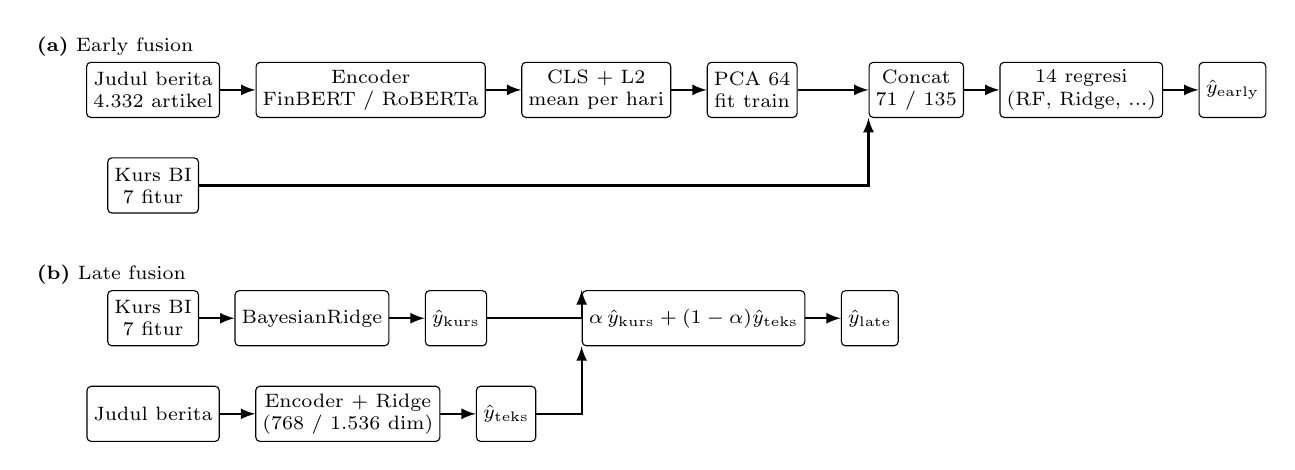
\begin{tikzpicture}[font=\scriptsize,
  box/.style={draw,rounded corners=1.5pt,align=center,inner sep=2.4pt,minimum height=7mm},
  arr/.style={-latex,thick}, node distance=4.5mm]
% panel a
\node[box] (a1) at (0,0) {Judul berita\\4.332 artikel};
\node[box,right=of a1] (a2) {Encoder\\FinBERT / RoBERTa};
\node[box,right=of a2] (a3) {CLS + L2\\mean per hari};
\node[box,right=of a3] (a4) {PCA 64\\fit train};
\node[box,below=5mm of a1] (a5) {Kurs BI\\7 fitur};
\node[box,right=9mm of a4] (a6) {Concat\\71 / 135};
\node[box,right=of a6] (a7) {14 regresi\\(RF, Ridge, ...)};
\node[box,right=of a7] (a8) {\(\hat y_{\text{early}}\)};
\draw[arr] (a1)--(a2);
\draw[arr] (a2)--(a3);
\draw[arr] (a3)--(a4);
\draw[arr] (a4)--(a6);
\draw[arr] (a5.east) -| (a6.south west);
\draw[arr] (a6)--(a7);
\draw[arr] (a7)--(a8);
\node[anchor=west] at (-1.6,0.55) {\textbf{(a)} Early fusion};

% panel b
\node[box] (b1) at (0,-2.9) {Kurs BI\\7 fitur};
\node[box,right=of b1] (b2) {BayesianRidge};
\node[box,right=of b2] (b3) {\(\hat y_{\text{kurs}}\)};
\node[box,below=5mm of b1] (b4) {Judul berita};
\node[box,right=of b4] (b5) {Encoder + Ridge\\(768 / 1.536 dim)};
\node[box,right=of b5] (b6) {\(\hat y_{\text{teks}}\)};
\node[box,right=12mm of b3] (b7) {\(\alpha\,\hat y_{\text{kurs}}+(1-\alpha)\hat y_{\text{teks}}\)};
\node[box,right=of b7] (b8) {\(\hat y_{\text{late}}\)};
\draw[arr] (b1)--(b2);
\draw[arr] (b2)--(b3);
\draw[arr] (b4)--(b5);
\draw[arr] (b5)--(b6);
\draw[arr] (b3.east) -| (b7.north west);
\draw[arr] (b6.east) -| (b7.south west);
\draw[arr] (b7)--(b8);
\node[anchor=west] at (-1.6,-2.35) {\textbf{(b)} Late fusion};
\end{tikzpicture}
\caption{Skema fusion. Early fusion menggabungkan fitur sebelum regresi; late fusion menggabungkan prediksi model unimodal dengan bobot \(\alpha\) dari validasi.}
\label{fig:arsitektur}
\end{figure}

\section{Setup Eksperimen dan Optimasi}
Empat belas regresi dipakai dengan set yang sama di A, B, dan C: LinearRegression, Ridge, Lasso, ElasticNet, BayesianRidge, KNN, SVR, DecisionTree, RandomForest, ExtraTrees, AdaBoost, GradientBoosting, XGBoost, dan LightGBM. Parameter default dan \feat{SEED=42} dipakai agar perbandingan antarvarian tidak tercampur efek tuning yang berbeda. Pemilihan konfigurasi untuk tuning dilakukan pada RMSE validasi; Tabel~\ref{tab:ablasi} sendiri melaporkan model terbaik per varian pada data uji, sehingga angka itu bersifat deskriptif, bukan hasil pemilihan yang bisa diulang tanpa melihat uji.

Hyperparameter tuning dilakukan pada model terbaik per varian menurut validasi. Pencarian memakai \feat{GridSearchCV} dengan \feat{TimeSeriesSplit(5)} di dalam train, sehingga tidak ada informasi masa depan yang masuk ke proses pemilihan. Grid kecil dipakai: Ridge \(\alpha\in\{0.1,1,10,100\}\), Lasso dan ElasticNet pada orde \(10^{-4}\) sampai \(10^{-2}\), KNN \(k\in\{3,5,7,11,21\}\), RandomForest kedalaman \(\{3,5,\text{tak terbatas}\}\) dan \feat{min\_samples\_leaf} \(\{1,5\}\), serta XGBoost dan LightGBM dengan 300 pohon dan learning rate 0,03 atau 0,05.

Feature importance dihitung dengan permutation importance pada data validasi, 20 kali pengulangan, memakai penurunan RMSE sebagai skor. Validasi dipilih agar importance tidak dihitung pada data yang dipakai melaporkan performa akhir. Untuk Model C, nama fitur adalah komponen PCA (\feat{finbert\_pc1} sampai \feat{pc64}), sehingga importance menunjukkan komponen mana yang dipakai model, bukan kata atau topik tertentu.

\section{Hasil Ablasi}
Tabel~\ref{tab:ablasi} merangkum model terbaik per varian pada data uji. Model A menjadi acuan 0,002981. Penambahan lexicon (B) menurunkan RMSE sekitar 2,0\% pada B\_vader dan B\_lex, sedangkan LM saja hanya 0,6\%. Penambahan embedding (C) memberi penurunan terbesar ketika kedua encoder digabung: C\_combined mencapai 0,002835 atau 4,9\% lebih rendah daripada A, dengan DirAcc tertinggi 0,591. FinBERT sendirian masih lebih baik daripada A, sedangkan DistilRoBERTa sendirian tidak.

\begin{table}[h]
\centering\small
\caption{Model terbaik per varian pada data uji. \(\Delta\)RMSE dihitung terhadap Model A terbaik (KNN, RMSE 0,002981).}
\label{tab:ablasi}
\footnotesize
\setlength{\tabcolsep}{4pt}
\begin{tabular}{llrrrrr}
\toprule
Varian & Model & Fitur & RMSE & MAE & DirAcc & \(\Delta\)RMSE \\
\midrule
A & KNN & 7 & 0,002981 & 0,002315 & 0,528 & -- \\
B\_vader & LinearRegression & 13 & 0,002921 & 0,002229 & 0,500 & \(-2,0\%\) \\
B\_lm & BayesianRidge & 17 & 0,002964 & 0,002267 & 0,443 & \(-0,6\%\) \\
B\_lex & LinearRegression & 23 & 0,002921 & 0,002220 & 0,557 & \(-2,0\%\) \\
C\_finbert\_early & RandomForest & 71 & 0,002914 & 0,002225 & 0,545 & \(-2,2\%\) \\
C\_roberta\_early & RandomForest & 71 & 0,002999 & 0,002315 & 0,477 & \(+0,6\%\) \\
C\_combined & RandomForest & 135 & \textbf{0,002835} & \textbf{0,002143} & \textbf{0,591} & \(-4,9\%\) \\
C\_finbert\_late & blend \(\alpha=0{,}83\) & 775 & 0,002989 & 0,002288 & 0,455 & \(+0,3\%\) \\
C\_roberta\_late & blend \(\alpha=1{,}00\) & 775 & 0,002984 & 0,002294 & 0,415 & \(+0,1\%\) \\
C\_combined\_late & blend \(\alpha=0{,}97\) & 1.543 & 0,002981 & 0,002290 & 0,426 & \(+0,03\%\) \\
\bottomrule
\end{tabular}
\end{table}

Late fusion tidak memberi perbaikan. Untuk DistilRoBERTa, \(\alpha\) optimal adalah 1,00, artinya validasi memilih mengabaikan teks sepenuhnya; baris C\_roberta\_late karena itu identik dengan BayesianRidge pada Model A. Untuk FinBERT, \(\alpha=0{,}83\) masih menyisakan 17\% bobot teks, tetapi RMSE ujinya tetap lebih buruk daripada early fusion. Penyebabnya, model teks linear atas 768 dimensi hanya dilatih pada 836 baris dan tidak memiliki cukup data untuk menyaingi model kurs.

Tuning juga tidak memperbaiki hasil uji (Tabel~\ref{tab:tuning}). Pada B\_vader, pemilihan validasi menjatuhkan pilihan ke RandomForest yang kemudian memburuk di uji. Pada B\_lm dan B\_lex, Ridge \(\alpha=100\) hampir menyamai default. Untuk C, Ridge hasil tuning pada FinBERT lebih buruk, sedangkan RandomForest hasil tuning pada C\_combined sedikit lebih buruk daripada RandomForest default. Pola ini konsisten dengan validasi yang hanya 178 hari: hyperparameter yang menang di validasi belum tentu menang di uji.

\begin{table}[h]
\centering\small
\caption{Perbandingan model default dan hasil tuning pada data uji.}
\label{tab:tuning}
\begin{tabular}{llrrr}
\toprule
Varian & Konfigurasi terpilih & CV RMSE & Test RMSE & Perubahan \\
\midrule
B\_vader & RandomForest, depth 3, leaf 5 & 0,003935 & 0,002980 & \(+2,0\%\) \\
B\_lm & Ridge, \(\alpha=100\) & 0,003669 & 0,002963 & \(-0,05\%\) \\
B\_lex & Ridge, \(\alpha=100\) & 0,003673 & 0,002941 & \(+0,7\%\) \\
C\_finbert\_early & Ridge, \(\alpha=100\) & 0,003871 & 0,003020 & \(+4,6\%\) \\
C\_roberta\_early & RandomForest, depth 3, leaf 5 & 0,003777 & 0,002902 & \(-3,3\%\) \\
C\_combined & RandomForest, depth 3, leaf 5 & 0,003714 & 0,002884 & \(+1,7\%\) \\
\bottomrule
\end{tabular}
\end{table}

\section{Analisis Fitur, Ruang Embedding, dan Error}
Permutation importance pada B\_lex menempatkan \feat{vader\_title\_mean} (2,9e-5), \feat{vader\_title\_pos\_ratio} (2,1e-5), \feat{lm\_text\_litigious} (1,5e-5), \feat{lm\_title\_positive} (1,3e-5), dan \feat{lm\_title\_net} (1,0e-5) di urutan teratas. Artinya, selain polaritas judul, proporsi kata litigius pada isi berita ikut dipakai model. Pada C\_combined, komponen teratas adalah \feat{roberta\_pc35} (1,5e-5), \feat{finbert\_pc3} (6,4e-6), dan \feat{finbert\_pc27} (3,6e-6). Karena berupa komponen PCA, angka ini tidak bisa diterjemahkan langsung menjadi topik tertentu tanpa memeriksa muatan komponen. Keterbatasan ini jujur perlu disebut: importance menunjukkan \emph{di mana} sinyal berada, bukan \emph{apa} temanya.

Gambar~\ref{fig:tsne} memproyeksikan 329 hari bursa yang embedding judulnya tersedia, dibagi menjadi 15\% hari paling volatil dan 15\% paling tenang. Kedua kelompok bercampur di hampir seluruh bidang proyeksi. Tidak ada klaster yang terpisah berdasarkan volatilitas, sehingga embedding judul FinBERT, tanpa fine-tuning, belum menghasilkan pemisahan linier yang jelas antara hari tenang dan hari bergejolak.

Analisis error membandingkan prediksi C\_combined (RandomForest) dengan Model A (KNN) pada 176 hari uji yang targetnya tidak nol. Model C membalik arah yang salah menjadi benar pada 47 hari, tetapi juga merusak arah yang tadinya benar pada 36 hari. Contoh perbaikan terbesar terjadi pada 18 Mei 2026 (target 0,00967, A memprediksi \(-0,00093\), C memprediksi 0,00048) dan 10 Agustus 2026 (target \(-0,00661\), A mendekati nol, C negatif). Perbaikan terbesar justru terjadi pada hari dengan return besar, yang menunjukkan model C lebih berani memberi arah saat sinyal teks kuat, tetapi keberanian yang sama juga menambah error di hari lain.

\begin{figure}[H]
\centering
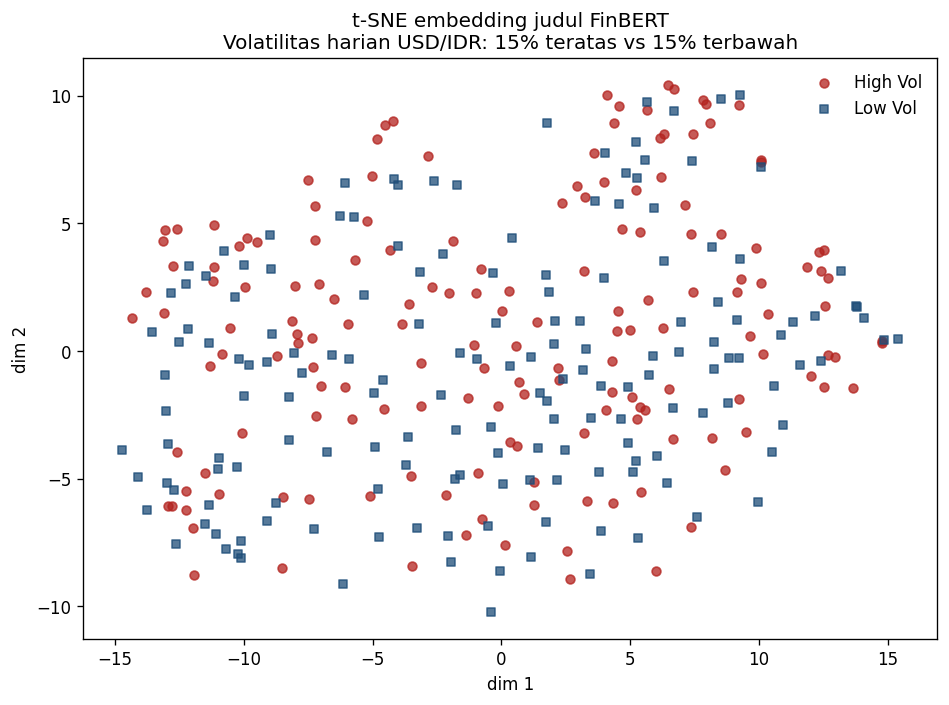
\includegraphics[width=0.62\linewidth]{../results/tsne_finbert.png}
\caption{t-SNE embedding judul FinBERT. Titik merah adalah 15\% hari dengan \(|r_t|\) terbesar, titik biru 15\% terkecil. Kedua kelompok tumpang tindih.}
\label{fig:tsne}
\end{figure}

\section{Keterbatasan dan Kesimpulan}
Tiga keterbatasan perlu dinyatakan. Pertama, baseline ``prediksi 0'' menghasilkan RMSE uji 0,002908, lebih baik daripada Model A (0,002981). Model C baru mengalahkan baseline itu sekitar 2,5\%, jadi klaim bahwa teks memberi nilai tambah harus dibaca sebagai perbaikan relatif antarvarian, bukan sebagai model yang siap dipakai. Kedua, laporan memilih model terbaik per varian berdasarkan data uji pada Tabel~\ref{tab:ablasi}; angka itu karena itu bersifat deskriptif dan sedikit optimistis. Ketiga, hasil bergantung pada satu seed. Perbedaan antara B\_lex (0,002921) dan C\_combined (0,002835) sekitar 3\%, cukup kecil sehingga variasi seed bisa mengubah urutan.

Kesimpulan yang didukung data: (1) fitur transformer menambah informasi di luar tujuh fitur kurs, dengan penurunan RMSE terbesar ketika dua encoder digabung; (2) early fusion lebih efektif daripada late fusion pada ukuran data ini; (3) tuning hyperparameter tidak menjamin perbaikan karena validasi terlalu pendek; dan (4) ruang embedding judul belum memisahkan rezim volatilitas secara visual. Pekerjaan lanjutan yang paling menjanjikan adalah fine-tuning encoder dengan regularisasi kuat, agregasi berbobot waktu (exponential decay), dan evaluasi lintas seed untuk mengukur stabilitas selisih antarvarian.

\begin{thebibliography}{9}
\small
\bibitem{araci} D. Araci, ``FinBERT: Financial Sentiment Analysis with Pre-trained Language Models,'' arXiv:1908.10063, 2019.
\bibitem{sanh} V. Sanh, L. Debut, J. Chaumond, T. Wolf, ``DistilBERT, a distilled version of BERT: smaller, faster, cheaper and lighter,'' arXiv:1910.01108, 2019.
\bibitem{hutto} C. Hutto dan E. Gilbert, ``VADER: A Parsimonious Rule-based Model for Sentiment Analysis of Social Media Text,'' ICWSM, 2014.
\bibitem{lm} T. Loughran dan B. McDonald, ``When Is a Liability Not a Liability? Textual Analysis, Dictionaries, and 10-Ks,'' Journal of Finance, 66(1), 2011.
\end{thebibliography}

\end{document}
